\section{RQ2: The Effect of Synchronization}
\label{sec:rq2}

\subsection{Shared atomics do not scale anywhere}

At $k \leq 16$ the atomic histogram is slower with eight threads than with
one in every environment: its speedup at $N=8$ is between 0.36 and 0.70
(Table~\ref{tab:speedup}). Natively it takes 380~ms on one thread at every
$k$ and 856, 864, 544 and 415~ms on eight at $k=1$, 4, 16 and 256
(Table~\ref{tab:times}); the local control takes 3.4 to 19.5~ms on eight.
At $N=8$ the shared counters cost 44 to 160 times the control natively.
This is the textbook cost of true sharing, and it is the same story in the
three environments. RQ2 asks something narrower: whether that cost,
relative to the control, differs between a browser and native code.

\subsection{The primary result}

\begin{table}[htbp]
\caption{Primary RQ2 contrasts at $N=8$: $\exp(\Delta r)$, the atomic/local
time ratio in the browser over the same ratio natively, with Bonferroni
99.5\% intervals. Bold: rejected by Holm ($\alpha=0.05$, 10 contrasts).
From Table~\ref{tab:primary}.}
\label{tab:rq2}
\centering\small
\begin{tabular}{lcc}
\toprule
$k$ & Chrome [99.5\% CI] & Firefox [99.5\% CI] \\
\midrule
1 & \textbf{2.26} [2.11, 2.41] & 1.01 [0.96, 1.07] \\
4 & \textbf{1.77} [1.75, 1.79] & \textbf{0.97} [0.96, 0.98] \\
16 & \textbf{1.43} [1.40, 1.45] & \textbf{0.83} [0.82, 0.84] \\
256 & \textbf{0.42} [0.41, 0.43] & \textbf{0.80} [0.78, 0.81] \\
\bottomrule
\end{tabular}
\end{table}

Table~\ref{tab:rq2} is the answer in the plan's metric, and
Figures~\ref{fig:rq2-ends} and~\ref{fig:rq2} draw the ratio
$T_{\mathrm{atomic}}/T_{\mathrm{local}}$ against $N$.
\begin{itemize}[leftmargin=1.5em]
\item \emph{Chrome.} When contention is concentrated on a few counters,
synchronization costs 1.4 to 2.3 times what it costs natively (2.26 at
$k=1$, 1.77 at $k=4$, 1.43 at $k=16$). When it is spread over 256 counters
it costs 0.42 times, and Chrome's atomic histogram even scales: a speedup
of 1.96 at $N=8$ against 0.92 natively and 0.97 in Firefox. The effect
changes sign with $k$.
\item \emph{Firefox} is never worse than native: no detectable difference
at $k=1$ (1.01, an interval of $\pm6$\%), and lower ratios from $k=4$ on
(0.97, 0.83, 0.80).
\end{itemize}
Seven of the eight contrasts are rejected; the smallest rejected effect,
Firefox at $k=4$, is 3\%.

\begin{figure}[htbp]
\centering
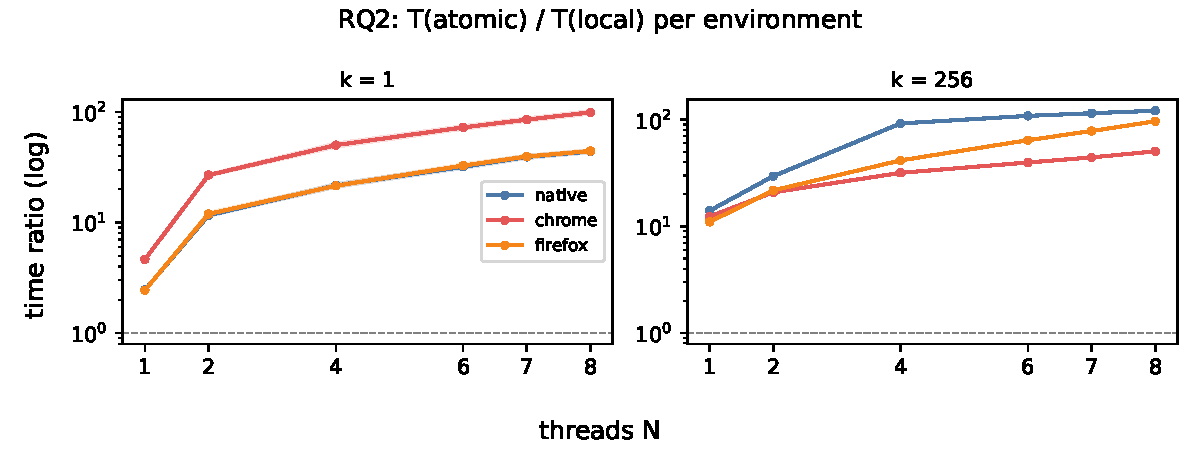
\includegraphics[width=0.8\linewidth]{../figures/campaign-rq2-ends.pdf}
\caption{RQ2: $T_{\mathrm{atomic}}/T_{\mathrm{local}}$ against $N$ at the
two ends of the sweep (log scale, 95\% CI).}
\Description{Atomic over local time ratio against thread count at k = 1 and k = 256, per environment.}
\label{fig:rq2-ends}
\end{figure}

\begin{figure}[htbp]
\centering
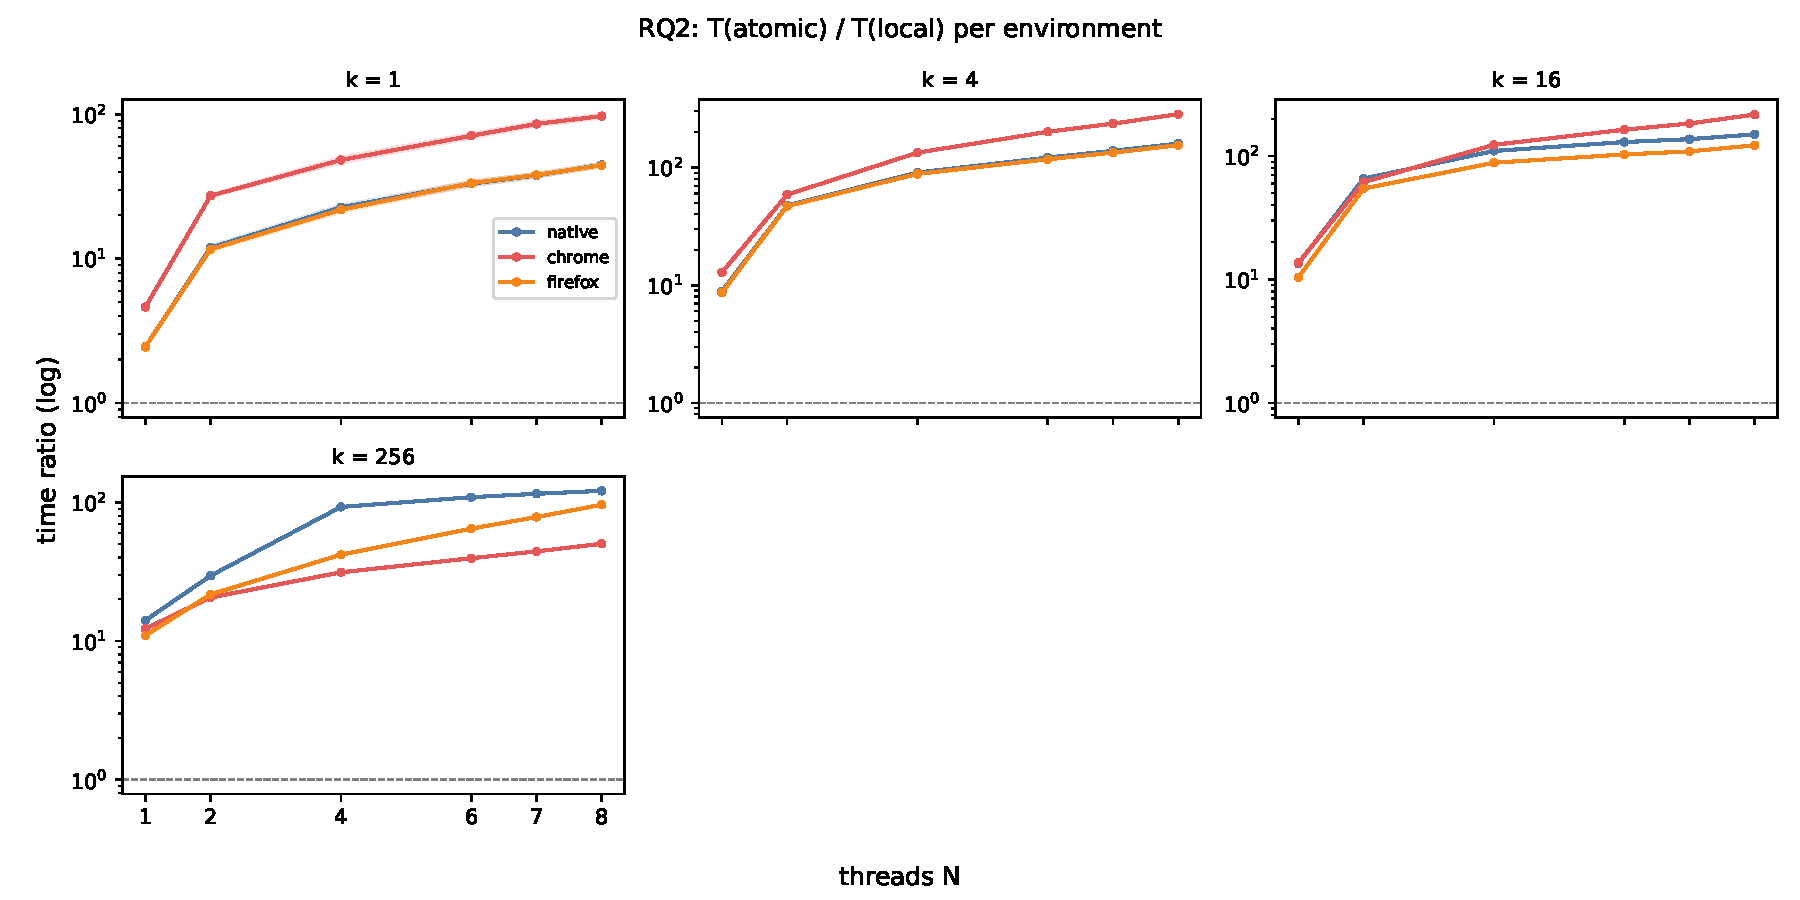
\includegraphics[width=\linewidth]{../figures/campaign-rq2.pdf}
\caption{RQ2: $T_{\mathrm{atomic}}/T_{\mathrm{local}}$ against $N$ for the
four values of $k$.}
\Description{Atomic over local time ratio against thread count for k = 1, 4, 16 and 256, per environment.}
\label{fig:rq2}
\end{figure}

\subsection{Every \texorpdfstring{$N$}{N}}

Table~\ref{tab:rq2-all} gives $\exp(\Delta r)$ for every thread count
(exploratory). Two things stand out. Part of Chrome's penalty exists
already with one thread: 1.89 at $k=1$ and 1.45 at $k=4$ with $N=1$, where
nothing is contended. At $k=1$ the atomic/local time ratio on one thread is
4.6 in Chrome against 2.5 natively and 2.4 in Firefox. So Chrome's effect
is a cost per operation as well as a cost of contention, which is what
Section~\ref{sec:why-rq2} finds in the machine code. And at $k=256$ both
browsers fall below 1 as soon as there are two threads, most at $N=4$
(Chrome 0.34, Firefox 0.45), because native code is at its worst there
(speedup 0.59 at $N=4$, Table~\ref{tab:speedup}).

\begin{table}[htbp]
\caption{Main campaign: the RQ2 effect $\exp(\Delta r)$ for every $k$ and $N$, with its 95\,\% bootstrap interval. Only $N=8$ is primary.}\label{tab:rq2-all}
\centering\small
\begin{tabular}{llcc}
\toprule
$k$ & $N$ & Chrome & Firefox \\
\midrule
1 & 1 & 1.89 [1.889, 1.891] & 0.9957 [0.9956, 0.9959] \\
1 & 2 & 2.313 [2.246, 2.379] & 1.029 [0.9891, 1.071] \\
1 & 4 & 2.319 [2.19, 2.461] & 0.9943 [0.9472, 1.043] \\
1 & 6 & 2.272 [2.16, 2.391] & 1.027 [0.9779, 1.076] \\
1 & 7 & 2.176 [2.072, 2.284] & 1.008 [0.9661, 1.053] \\
1 & 8 & 2.259 [2.157, 2.365] & 1.01 [0.9724, 1.049] \\
\midrule
4 & 1 & 1.45 [1.447, 1.454] & 0.977 [0.9763, 0.9777] \\
4 & 2 & 1.264 [1.244, 1.284] & 0.993 [0.9777, 1.009] \\
4 & 4 & 1.473 [1.457, 1.49] & 0.978 [0.9663, 0.9903] \\
4 & 6 & 1.651 [1.635, 1.669] & 0.96 [0.9493, 0.971] \\
4 & 7 & 1.722 [1.705, 1.739] & 0.9777 [0.9669, 0.9881] \\
4 & 8 & 1.771 [1.754, 1.787] & 0.9691 [0.9597, 0.9788] \\
\midrule
16 & 1 & 1.034 [1.031, 1.038] & 0.786 [0.7839, 0.7881] \\
16 & 2 & 0.9486 [0.9385, 0.959] & 0.8446 [0.8355, 0.8538] \\
16 & 4 & 1.14 [1.126, 1.154] & 0.8189 [0.8071, 0.8306] \\
16 & 6 & 1.266 [1.256, 1.277] & 0.7989 [0.792, 0.806] \\
16 & 7 & 1.344 [1.33, 1.359] & 0.8 [0.7932, 0.8067] \\
16 & 8 & 1.425 [1.408, 1.442] & 0.8311 [0.824, 0.8385] \\
\midrule
256 & 1 & 0.881 [0.8732, 0.8857] & 0.786 [0.771, 0.7966] \\
256 & 2 & 0.7061 [0.6995, 0.7103] & 0.7359 [0.7266, 0.7439] \\
256 & 4 & 0.3442 [0.341, 0.3473] & 0.4502 [0.445, 0.4553] \\
256 & 6 & 0.3654 [0.3613, 0.37] & 0.5918 [0.5861, 0.5979] \\
256 & 7 & 0.3852 [0.3823, 0.388] & 0.681 [0.6755, 0.6865] \\
256 & 8 & 0.4159 [0.4096, 0.4222] & 0.7965 [0.7864, 0.8058] \\
\bottomrule
\end{tabular}
\end{table}


\subsection{The two factors of the ratio}
\label{sec:decomposition}

$\exp(\Delta r)$ is a ratio of ratios:
\[
\exp(\Delta r) = \frac{A_b/A_n}{L_b/L_n},
\]
with $A$ the time of the atomic histogram, $L$ of the local one, $b$ a
browser and $n$ native. At $N=8$ the local kernel is about 1\% of the
atomic time, yet its own environment gap $L_b/L_n$ divides the result with
full weight: a browser whose local kernel is slower than native's gets a
lower $\exp(\Delta r)$ even if its atomics cost exactly what native's do.
The ratio is therefore always read with its two factors
(Table~\ref{tab:decomposition}), which tell the two engines apart.

\begin{table}[htbp]
\caption{The two factors of each primary RQ2 ratio at $N=8$ (post hoc, 95\,\% intervals): the atomic time and the local time in the browser over native, and the ratio of the excesses $(A_b-L_b)/(A_n-L_n)$.}\label{tab:decomposition}
\centering\footnotesize
\begin{tabular}{llcccc}
\toprule
Browser & $k$ & $\exp(\Delta r)$ & Atomic $A_b/A_n$ & Local $L_b/L_n$ & Excess \\
\midrule
Chrome & 1 & 2.259 [2.157, 2.365] & 2.206 [2.105, 2.308] & 0.9762 [0.9755, 0.977] & 2.234 [2.131, 2.34] \\
Chrome & 4 & 1.771 [1.754, 1.787] & 1.909 [1.892, 1.925] & 1.078 [1.074, 1.082] & 1.914 [1.897, 1.93] \\
Chrome & 16 & 1.425 [1.408, 1.442] & 1.78 [1.772, 1.788] & 1.249 [1.235, 1.264] & 1.784 [1.775, 1.792] \\
Chrome & 256 & 0.4159 [0.4096, 0.4222] & 0.5074 [0.5068, 0.508] & 1.22 [1.202, 1.239] & 0.5015 [0.5009, 0.5021] \\
Firefox & 1 & 1.01 [0.9724, 1.049] & 1.026 [0.9875, 1.066] & 1.015 [1.014, 1.017] & 1.026 [0.9868, 1.067] \\
Firefox & 4 & 0.9691 [0.9597, 0.9788] & 0.9837 [0.9751, 0.9926] & 1.015 [1.011, 1.019] & 0.9835 [0.9748, 0.9925] \\
Firefox & 16 & 0.8311 [0.824, 0.8385] & 1.007 [1.002, 1.013] & 1.212 [1.204, 1.22] & 1.006 [1.001, 1.011] \\
Firefox & 256 & 0.7965 [0.7864, 0.8058] & 0.9479 [0.9468, 0.949] & 1.19 [1.176, 1.205] & 0.9459 [0.9448, 0.947] \\
\bottomrule
\end{tabular}
\end{table}


\begin{itemize}[leftmargin=1.5em]
\item \emph{Chrome's effect is in the numerator.} Its atomic histogram
takes 2.21, 1.91 and 1.78 times the native time at $k=1$, 4 and 16, and
0.51 times at $k=256$; its local kernel is within 0.98 to 1.25 of native.
$\exp(\Delta r)$ falls from 2.26 to 1.43 between $k=1$ and 16 mostly
because Chrome's local kernel gets slower relative to native as $k$ grows,
while the atomic ratio stays near 2.
\item \emph{Firefox's effect is in the denominator.} Its atomic times are
the native ones (1.03, 0.98, 1.01 and 0.95 times) and its local histogram
is 1.21 and 1.19 times slower at $k=16$ and 256. ``Synchronization is
relatively cheaper in Firefox'' at $k \geq 16$ is true of the ratio and
misleading as a statement about synchronization.
\end{itemize}
The last column answers RQ2 in absolute terms, the time the shared counters
add in the browser over the time they add natively: about 2.2, 1.9 and 1.8
times in Chrome at $k \leq 16$ and 0.50 times at $k=256$; in Firefox 1.03,
0.98, 1.01 and 0.95. The two readings tell the same story for Chrome. For
Firefox they differ most at $k=16$: 0.83 by the ratio, 1.006 [1.001, 1.011]
by the excess.

\subsection{Robustness and sensitivity}

\begin{table}[htbp]
\caption{Robustness of the ten primary contrasts: Mann-Whitney $U$ and Cliff's $\delta$ on per-run ratios, Holm-adjusted, the share of 1000 random re-pairings with the same decision, and the agreement with the bootstrap decision.}\label{tab:robustness}
\centering\footnotesize
\begin{tabular}{lllrrrrlrl}
\toprule
RQ & Browser & Cell & $\delta$ & $U$ & $p$ & Holm $p$ & Rej. & Share & Agree \\
\midrule
RQ2 & Chrome & atomic, $k$=1 & 1 & 900 & 3.02e-11 & 3.02e-10 & yes & 1 & yes \\
RQ2 & Chrome & atomic, $k$=4 & 1 & 900 & 3.02e-11 & 3.02e-10 & yes & 1 & yes \\
RQ2 & Chrome & atomic, $k$=16 & 1 & 900 & 3.02e-11 & 3.02e-10 & yes & 1 & yes \\
RQ2 & Chrome & atomic, $k$=256 & -1 & 0 & 3.02e-11 & 3.02e-10 & yes & 1 & yes \\
RQ2 & Firefox & atomic, $k$=1 & 0.05778 & 476 & 0.7062 & 0.7062 & no & 1 & yes \\
RQ2 & Firefox & atomic, $k$=4 & -0.74 & 117 & 8.841e-07 & 2.652e-06 & yes & 1 & yes \\
RQ2 & Firefox & atomic, $k$=16 & -1 & 0 & 3.02e-11 & 3.02e-10 & yes & 1 & yes \\
RQ2 & Firefox & atomic, $k$=256 & -1 & 0 & 3.02e-11 & 3.02e-10 & yes & 1 & yes \\
RQ1 & Chrome & filter & -0.2444 & 340 & 0.1055 & 0.2109 & no & 0.999 & yes \\
RQ1 & Firefox & filter & 0.9244 & 866 & 8.097e-10 & 3.239e-09 & yes & 1 & yes \\
\bottomrule
\end{tabular}
\end{table}

\begin{table}[htbp]
\caption{The plan's sensitivity checks on the ten primary contrasts (effect with its 99.5\,\% interval): as planned, with the per-run mean, with the median across runs, and with no foreign-CPU exclusion. A decision that changes under a check would be marked not robust.}\label{tab:sensitivity}
\centering\footnotesize
\begin{tabular}{llcccl}
\toprule
Browser & Cell & As planned & Per-run mean & Median centre & Robust \\
\midrule
Chrome & atomic, $k$=1 & 2.259 [2.11, 2.406] & 2.259 [2.111, 2.406] & 2.397 [1.989, 2.512] & yes \\
Chrome & atomic, $k$=4 & 1.771 [1.746, 1.793] & 1.765 [1.736, 1.795] & 1.766 [1.741, 1.798] & yes \\
Chrome & atomic, $k$=16 & 1.425 [1.399, 1.451] & 1.429 [1.397, 1.461] & 1.419 [1.4, 1.452] & yes \\
Chrome & atomic, $k$=256 & 0.4159 [0.4072, 0.4251] & 0.4158 [0.4066, 0.4256] & 0.4146 [0.4028, 0.4279] & yes \\
Firefox & atomic, $k$=1 & 1.01 [0.9573, 1.067] & 0.994 [0.9408, 1.049] & 1.053 [0.9509, 1.111] & yes \\
Firefox & atomic, $k$=4 & 0.9691 [0.9555, 0.9827] & 0.9727 [0.9577, 0.9885] & 0.9671 [0.9512, 0.9854] & yes \\
Firefox & atomic, $k$=16 & 0.8311 [0.8208, 0.8417] & 0.8385 [0.825, 0.8525] & 0.83 [0.8155, 0.8458] & yes \\
Firefox & atomic, $k$=256 & 0.7965 [0.782, 0.8089] & 0.7992 [0.7821, 0.8139] & 0.8046 [0.7862, 0.8177] & yes \\
Chrome & filter & 0.9955 [0.9868, 1.004] & 0.9936 [0.984, 1.003] & 0.9953 [0.9807, 1.009] & yes \\
Firefox & filter & 1.055 [1.034, 1.072] & 1.037 [1.015, 1.055] & 1.051 [1.037, 1.071] & yes \\
\bottomrule
\end{tabular}
\end{table}


Mann-Whitney agrees with the bootstrap decision on all ten primary
contrasts (Table~\ref{tab:robustness}). The eight rejected ones have
$|\delta| \geq 0.74$, six of them $|\delta| = 1$: every browser run is on
one side of every native run. The two not rejected have $p = 0.11$ (Chrome,
RQ1) and $p = 0.71$ (Firefox, $k=1$). The decision is the same in at least
99.9\% of 1000 random re-pairings of the runs. All ten decisions also hold
under the plan's three sensitivity checks (Table~\ref{tab:sensitivity}):
the per-run mean, the median across runs (which widens Chrome's interval at
$k=1$ to [1.99, 2.51], the cell whose runs fall on levels) and no exclusion
threshold (identical, since no run was excluded).
